\chapter{Time-independent Schr\"odinger equation}

\section{Stationary states}
How do we get $\Psi \left( x,t \right)$ in first place.
We first consider the potential is independent of $t$, then
\begin{equation}
  \label{eq:2-1}
i \hbar \frac{\partial \Psi}{\partial t} = - \frac{\hbar^{2}}{2m} \frac{\partial^{2} \Psi}{\partial x^2} + V \Psi.
\end{equation}
In this case, the Schr\"odinger equation can be solved by the method of \textbf{separation of variables}.
We look for solutions that are simple porducts
\begin{equation}
  \label{eq:2-2}
  \Psi \left( x,t \right) = \psi \left( x \right) \phi \left( t \right)
\end{equation}
Of course, we cannot hope to get more than a tiny subset of all solutions in this way.
But the solution we got turn out to be of great interest.
Moreover we will be able at the end to patch together the sparable solutions in such a way as to construct the most general solution.

For separabel solution we have
\begin{equation}
  \label{eq:2-3}
  i\hbar \frac{1}{\phi} \frac{\dd \phi}{\dd t} = - \frac{\hbar^{2}}{2m} \frac{1}{\psi} \frac{\dd^{2} \psi}{\dd x^{2}} + V.
\end{equation}
Now, in Eq.~\eqref{eq:2-3}, the left side is only $t$ dependent and the right side is a function of $x$ alone.
The only with this can be true is if both sides are in fact a constant, we denote it $E$.
\begin{align}
  \label{eq:2-4}
  \frac{\dd \phi}{\dd t} &= - \frac{i E}{\hbar} \phi \\
  \label{eq:2-5}
  -\frac{\hbar^{2}}{2m} \frac{\dd^{2}\psi}{\dd x^{2}} + V\psi &= E\psi
\end{align}
Separation of variables turns the partial differential equation into two ordinary differential equations.
For Eq.~\eqref{eq:2-4}, the solution is easy to give
\begin{equation}
  \label{eq:2-6}
  \phi \left( x,t \right)  = e^{-i Et/\hbar}.
\end{equation}
The Eq.~\eqref{eq:2-5} is called the \textbf{time-independent Schr\"odinger equation}.

There are several advangates to do the separable solution in Eq.~\eqref{eq:2-2}.

\textbf{1.} They are \textbf{stationary states}.
Although the wave function dependent on $t$ as suggested in Eq.~\eqref{eq:2-6}, the probability density does not.
The same thing happens in calculating the expectation value of any dynamical variable.
The Eq.~\eqref{eq:1-18} become
\begin{equation}
  \label{eq:2-7}
  \expval{ Q \left( x,p \right) } = \int \psi^{*} Q \left( x, \frac{\hbar}{i} \frac{\dd}{\dd x} \right) \psi \dd x.
\end{equation}
Thus every expectation value is constant in time.

\textbf{2.} Teh are states of definite total energy.
In calassica mechanics, the total energy is called the \textbf{Hamiltonian}.
The cooresponding operator is
\begin{equation}
  \label{eq:2-8}
  \hat{H} = - \frac{\hbar^{2}}{2m} \frac{\partial^{2}}{\partial x^{2}} + V \left( x \right).
\end{equation}
Then the time-independent Schr\"odinger equation can be written
\begin{equation}
  \label{eq:2-9}
  \hat{H} \psi = E\psi
\end{equation}
One can calculate the variance of $H$ which is $\sigma_{H}^{2}=0$.
This means a separable solution has the property that every measurement of the total energy is certain to return the value $E$.

\textbf{3.} The general suolution is a \textbf{linear combination} of separable solution.
\begin{equation}
  \label{eq:2-10}
  \Psi \left( x,t \right) = \sum_{n=1}^{\infty} c_{n} \psi_{n} \left( x \right) e^{-i E_{n}t /\hbar}.
\end{equation}

Last comment, even the separable suolutions themselves are statinary state, their linearly combination Eq.~\eqref{eq:2-10} are usually not.

\begin{fullwidth}
  \hrulefill\\
  \textbf{Problem} Prove the following theorems
  \begin{itemize}
    \item For normalizable solutions, the separation constant $E$ must be real.
    \item THe time-independent wave function $\psi \left( x \right)$ can always be taken to be real.
    \item If $V \left( x \right)$ is an even function then $\psi \left( x \right)$ can always be taken to either even or odd
  \end{itemize}

  \textbf{Problem} Show that $E$ must exceed the minimum value of $V \left( x \right)$ for every normalizable solution to the time-independent Schr\"odinger equation.
  \\ \hrulefill
\end{fullwidth}

\section{The infinite square well}
Suppose the potential is
\begin{equation}
  \label{eq:2-11}
  V \left( x \right) =
  \begin{cases}
    0 ~ & \text{if $0 \leq x \leq a$}, \\
    \infty  ~ & \text{otherwise}.
  \end{cases}
\end{equation}
A particle in this potential is complete free, except at the two end point, where an infinite force prevents it from escaping as shown in Fig.~\ref{fig:2-1}.
\begin{figure}[h]
  \centering
  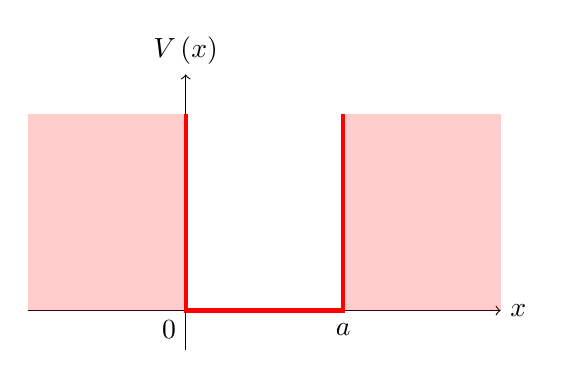
\begin{tikzpicture}
    \draw [black,->] (0,-0.5) -- (0,3);
    \draw [black,->] (-2,0) -- (4,0);
    \node [right] at (4,0) {$x$};
    \node [above] at (0,3) {$V\left(x\right)$};
    \draw [red, line width = 1.5] (0,2.5) -- (0,0) -- (2,0) -- (2,2.5);
    \node [below] at (2,-0.04) {$a$};
    \node [below left] at (0,0) {$0$};
    \fill [red, opacity=0.2] (0,0) rectangle (-2,2.5);
    \fill [red, opacity=0.2] (2,0) rectangle (4,2.5);
  \end{tikzpicture}
  \label{fig:2-1}
  \caption{The infinite square well potential.}
\end{figure}

Outside the well, $\psi \left( x \right)=0$, since you can not have a particel with infinte high energy.
Inside the well, we have
\begin{equation}
  \label{eq:2-12}
  \frac{\dd^{2} \psi}{\dd x^{2}}  = -k^{2} \psi, ~ ~  \text{where } k= \frac{\sqrt{2mE}}{\hbar}.
\end{equation}
This is the classical \textbf{simple harmonic oscillator} equation; the general solution is
\begin{equation}
  \label{eq:2-13}
  \psi \left( x \right) = A \sin kx + B \cos kx
\end{equation}
where $A$ and $B$ are arbitary constants.



%%% Local Variables:
%%% mode: latex
%%% TeX-master: "main"
%%% End:
